\documentclass[12pt]{article}
\usepackage[margin=2cm]{geometry}
\usepackage{cite}
\usepackage{float}
\usepackage{graphicx}
\usepackage[caption=false]{subfig}
  \DeclareGraphicsExtensions{.png}
\usepackage{amsmath}
\usepackage{amsfonts}
\usepackage{url}
\usepackage{tikz}
\usetikzlibrary{shapes,shapes.gates.logic.US,arrows,chains,calc}
\tikzset{
  -|-/.style={
    to path={
      (\tikztostart) -| ($(\tikztostart)!#1!(\tikztotarget)$) |- (\tikztotarget)
      \tikztonodes
    }
  },
  -|-/.default=0.5,
  |-|/.style={
    to path={
      (\tikztostart) |- ($(\tikztostart)!#1!(\tikztotarget)$) -| (\tikztotarget)
      \tikztonodes
    }
  },
  |-|/.default=0.5,
}
\usepackage{tikz-timing}
\usetikztiminglibrary[new={char=Q,reset char=R}]{counters}
\usepackage{bm,times}
\usepackage{pgfgantt}
\usepackage{indentfirst}
\usepackage{array}

\begin{document}
\begin{titlepage}
  { \Large
    Imperial College London\\[17pt]
    Department of Electrical and Electronic Engineering\\[17pt]
    Final Year Project Report \textcolor{red}{[DRAFT]}
  }

  \rule{\columnwidth}{3pt}
  \vfill
  \centering
  \includegraphics[width=0.7\columnwidth]{img/1.jpg}
  \vfill

  \begin{table}[h]
  \def\arraystretch{1.8}
    \begin{tabular}{p{40mm}p{\dimexpr\columnwidth-40mm}}
      Project Title: & \textbf{An Extensible Framework for \newline At-speed Evaluation of Arithmetic Hardware} \\
      Student:       & \textbf{Zifan Wang} \\
      CID:           & \textbf{01077639} \\
      Course:        & \textbf{EEE4} \\
      Project Supervisor: & \textbf{Dr. James J. Davis} \\
      Second Marker: & \textbf{Dr. Christos Bouganis}
    \end{tabular}
  \end{table}
\end{titlepage}

% \markboth{2018-2019}{?}
\setcounter{tocdepth}{2}
\tableofcontents

\newpage

\begin{abstract}
  Nice abstract
\end{abstract}

\section{Introduction}

\section{Background}

\section{Requirements Capture}

\section{System-level Design}

\subsection{Testbench Architecture}
\subsection{User Interface}

\section{Hardware Design Choices}


\subsection{Randomiser}
With relatively low effort, random testing can provide significant coverage and discover relatively subtle errors~\cite{Duran1}.
LFSRs are a reliable way of generating pseudorandom numbers quickly with low cost~\cite{Hazwani1}.
\subsubsection{LFSR Configurations}

An 8-bit LFSR has taps at [8,6,5,4].

\textit{Fibonacci} --
Classical option, easier to write and scale in hardware.

\begin{figure}[ht]
  \centering
  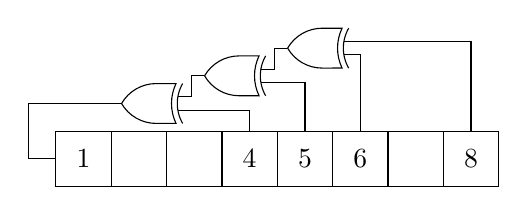
\begin{tikzpicture}
  [
    x=1em, y=1em,
    start chain = going right,
    node distance = 0em,
    reg/.style =
      {draw, minimum width=2em, minimum height=2em,outer sep=0pt, on chain},
    every join/.style={-, thick}
  ]
  \node [reg] at (0, 0) (1) {1};
  \node [reg] (2) {};
  \node [reg] (3) {};
  \node [reg] (4) {4};
  \node [reg] (5) {5};
  \node [reg] (6) {6};
  \node [reg] (7) {};
  \node [reg] (8) {8};

  \node[xor gate US,draw,rotate=180] at (2.5, 2) (a) {};
  \node[xor gate US,draw,rotate=180] at (5.5, 3) (b) {};
  \node[xor gate US,draw,rotate=180] at (8.5, 4) (c) {};

  \draw (4.north)  |- (a.input 1);
  \draw (5.north)  |- (b.input 1);
  \draw (6.north)  |- (c.input 1);

  \draw (b.output) to[-|-] (a.input 2);
  \draw (c.output) to[-|-] (b.input 2);
  \draw (8.north)       |- (c.input 2);

  \draw (a.output) -- (-2, 2) |- (1.west);

\end{tikzpicture}
  \caption{Fibonacci Configuration}
  \label{FibLFSR}
\end{figure}

\textit{Galois} --
Harder to write if variable length is desired, but faster in hardware.

\begin{figure}[ht]
  \centering
  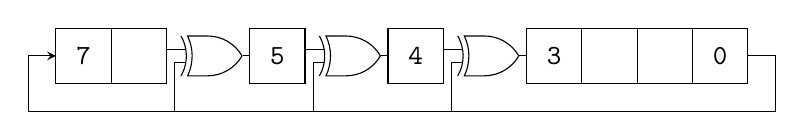
\begin{tikzpicture}
  [
    x=1em, y=1em,
    start chain = going left,
    node distance = 0em,
    reg/.style =
      {draw, minimum width=2em, minimum height=2em, outer sep=0pt, on chain},
    spa/.style =
      {minimum width=3em, minimum height=2em, outer sep=0pt, on chain},
    every join/.style={-, thick}
  ]
  \node [reg] at (0, 0) (1) {\texttt{0}};
  \node [reg] (2) {};
  \node [reg] (3) {};
  \node [reg] (4) {\texttt{3}};
  \node [spa] ()  {};
  \node [reg] (5) {\texttt{4}};
  \node [spa] ()  {};
  \node [reg] (6) {\texttt{5}};
  \node [spa] ()  {};
  \node [reg] (7) {};
  \node [reg] (8) {\texttt{7}};

  \node [xor gate US,draw] at  (-8.4, 0) (a) {};
  \node [xor gate US,draw] at (-13.4, 0) (b) {};
  \node [xor gate US,draw] at (-18.4, 0) (c) {};

  \draw [->, >=stealth] (1.east) -| (2, -2) -- (-25,-2) |- (8.west);

  \draw (a.input 1-|5.east) -- (a.input 1);
  \draw (b.input 1-|6.east) -- (b.input 1);
  \draw (c.input 1-|7.east) -- (c.input 1);

  \draw  (-9.7,-2) |- (a.input 2);
  \draw (-14.7,-2) |- (b.input 2);
  \draw (-19.7,-2) |- (c.input 2);

  \draw (a.output) -- (4.west);
  \draw (b.output) -- (5.west);
  \draw (c.output) -- (6.west);

\end{tikzpicture}
  \caption{Galois Configuration}
  \label{GalLFSR}
\end{figure}

\textit{Xorshift} --
Interesting, but seems quite bad in hardware~\cite{Marsaglia1}.

\subsubsection{LFSR Structure}

\textit{Vertical} --
Nice randomness, more scalable, need to seed all the LFSRs differently.

\textit{Horizontal} --
Easy to build, easy to test with.

\subsection{Driver}
\subsubsection{Dual Driver System}
One driver focusses on fast stress tests,
The other allows handwritten tests to coexist with random tests.
They can be switched in software.

\subsection{Monitor}


\subsection{Scoreboard}

\section{Software Design Choices}

\subsection{Code Structure}


\section{Hardware Implementation}

\subsection{Project Hierarchy}

\subsection{Randomiser}

\subsection{Driver}

\subsubsection{Delay Tester}

I built a delay tester to find out the delay of the DUT.
With a 3-bit counter as shown in the timing diagram, it can measure this delay for up to 8 clock cycles.

\begin{figure}[ht]
  \centering
  \begin{tikztimingtable}
  [
    xscale=2.5,
    timing/d/background/.style={fill=white},
    timing/font=\ttfamily
  ]
  out\_count       & 6R 2{Q} 0R 8{Q} 0R 8{Q} 0R Q\\
                   & L 2{H 7L}       HL          \\
  o\_drive         & U 2{D{0} 7U}    D{0}U       \\
  i\_dut\_out      & U 2{3U D{0} 4U} 2U          \\
  test\_state      & 5D{00} 5D{01} 3D{10} 6D{11} \\
  delay\_out       & 11D{0} D{1} D{2} 6D{3}      \\
\extracode
  % Add vertical lines in two colors
  \begin{pgfonlayer}{background}
    \begin{scope}[semitransparent,semithick]
      \vertlines{1,2,...,18}
    \end{scope}
  \end{pgfonlayer}
\end{tikztimingtable}
  \caption{3-bit Delay Tester FSM}
  \label{DelayTester}
\end{figure}
Testing with 0 is safe since LSFR will never output 0.

\subsubsection{Switching system}

\subsection{Monitor}
\subsubsection{Sub Monitors}

\begin{figure}[ht]
  \centering
  \begin{tikztimingtable}
    [
      xscale=4,
      timing/d/background/.style={fill=white},
      timing/font=\ttfamily
    ]
    dist\_ctr & D{8} 2{D{1}D{2}D{4}D{8}} D{1}D{2}         \\
    a & U D{AA}D{AB}D{AC}D{AD}D{AE}D{AF}D{AG}D{AH}D{AI} U \\
    b & U D{BA}D{BB}D{BC}D{BD}D{BE}D{BF}D{BG}D{BH}D{BI} U \\
    s & 3U D{SA}D{SB}D{SC}D{SD}D{[red]SK}D{SF}D{SG}D      \\
    \\
    dist\_ctr  [0] & L 2{H 3L} HL \\
    a\_mon     [0] & U 4D{AA} 4D{AE} 2D{AI} \\
    b\_mon     [0] & U 4D{BA} 4D{BE} 2D{BI} \\
    s\_mon     [0] & 2U 4D{SA} 4D{SE} D \\
    sub\_event [0] & 8LH2L \\
  \extracode
    % Add vertical lines in two colors
    \begin{pgfonlayer}{background}
      \begin{scope}[semitransparent,semithick]
        \vertlines{1,2,...,10}
      \end{scope}
    \end{pgfonlayer}
  \end{tikztimingtable}
  \caption{Distributed Monitoring System}
  \label{DisMon}
\end{figure}

\subsection{Scoreboard}

\section{Software Implementation}

\section{System Integration}

\subsection{Qsys}


\section{Testing}

\section{Results}

\section{Evaluation}

\section{Conclusion}

\section{Further Work}

\section{User Guide}

\newpage
\appendix

% \chapter{User Guide Provided to Test Volunteers}

\chapter{Raw Data}

\textcolor{red}{+Code Snippets?}


\input{tex/bibliography}

\end{document}